%
% Szakdolgozat minta az Eszterházy Károly Egyetem
% matematika illetve informatika szakos hallgatóinak.
%

\documentclass[
% opciók nélkül: egyoldalas nyomtatás, elektronikus verzió
% twoside,     % kétoldalas nyomtatás
% tocnopagenum,% oldalszámozás a tartalomjegyzék után kezdődik
]{thesis-ekf}
\usepackage[T1]{fontenc}
\PassOptionsToPackage{defaults=hu-min}{magyar.ldf}
\usepackage[magyar]{babel}
\usepackage{mathtools,amssymb,amsthm}
\usepackage{listings}
\usepackage{graphicx}
\usepackage{float}

\footnotestyle{rule=fourth}

\newtheorem{tetel}{Tétel}[chapter]
\theoremstyle{definition}
\newtheorem{definicio}[tetel]{Definíció}
\theoremstyle{remark}
\newtheorem{megjegyzes}[tetel]{Megjegyzés}

\begin{document}
\institute{Matematikai és Informatikai Intézet}
\title{A szakdolgozat címe}

%\author{Szerző neve\\szak}
\author{ Sass-Gyarmati Norbert\\Programtervező informatikus BSc
	\collaborator
	Oravecz Zsolt\\Programtervező informatikus BSc}
\supervisor{Dr. Geda Gábor\\Egyetemi docens}
\city{Eger}
\date{2021}
\maketitle
\tableofcontents

\chapter*{Bevezetés}
Megújuló energiaforrásnak nevezzük az energiahordozók azon csoportját, amelyek emberi időléptékben képesek megújulni, azaz nem fogynak el, ellentétben a nem megújuló energiaforrásokkal.  A mai civilizáció a zöld energiát helyezi előtérbe, és arra törekszik, hogy minél kisebbre csökkentse az ökológiai lábnyomot. Számos gyakorlati felhasználása van, többek között a villanyautók, tisztán elektromos hajtással működő személygépjárművek, illetve egyéb járművek fejlesztése. Napjainkban számos helyen tapasztaljuk, hogy egyre nagyobb szerepet kap a fenntarthatóság és a környezettudatosság nemcsak a vállalatok és cégek, hanem a fogyasztók gondolkodásában is. Egyre több szerepet kap az életünkben a környezettudatos életmód, a szelektív hulladékgyűjtés és a zöldebb életmód. Számos előnyökkel rendelkeznek a megújuló energiaforrások, például, hogy ezek hosszú távon rendelkezésre álló készletek, szemben a nem megújuló energiaforrásokkal, melyek fosszilis energiahordozók. A fosszilis energiahordozók nem tartanak örökké, hiszen ezeket a földből kinyerve nem lehet őket pótolni, ha már véglegesen elfogytak. Ide tartozik az urán, a kőolaj, földgáz, illetve a szén. Ezen kívül rendelkezik egy másik nagy előnnyel, hogy működésük rendkívül környezetkímélő. A fosszilis energiahordozók égetése hatalmas mennyiségű szén-dioxidot bocsát ki, ezzel mesterségesen növelve az üvegházhatás folyamatát a Földünkön, ezzel szemben a megújuló energiaforrások használatával sokkal kevesebb károsanyag kerül a légkörbe, melyeknek felhasználását egyre több ország helyezi előtérbe, hogy ezzel is mérsékelni tudják a globális felmelegedés problémáját.
\par Szakdolgozatunkban  a megújuló energiaforrások tudatos, és környezetvédő felhasználását szeretnénk modellezni.  A modellünkben az energiaforrásokat mikrokontrollerrel 
ötvözve szeretnénk a leghatékonyabban szabályozni intelligens módon, azaz a rendszer képes önállóan optimalizálni a termelt és a felhasznált energia mennyiségét. Gyakorlati felhasználásban terepasztalon elhelyezett kisméretű modelleken szemléltetjük a különféle erőműveket, illetve energiatároló technológiákat, fogyasztókat. Fogyasztóinknak gyakorlati felhasználásuk lesz, mely azt jelenti, hogy a való életben megtalálható általános fogyasztókkal fogjuk szimulálni a projektet. Ilyenek lehetnek a családi házak, háztömbök, elektromos töltőállomások, iskolák és gyárak.

\chapter{Tudományos Diákköri Konferencia}
	\section{Szakasz címe}
		\subsection{Alszakasz címe}
		Lórum ipse olyan borzasztóan cogális patás, ami fogás nélkül nem varkál megfelelően. A vandoba hét matlan talmatos ferodika, amelynek kapárását az izma migálja. A vandoba bulái közül ,,zsibulja'' meg az izmát, a pornát, valamint a művést és vátog a vandoba buláinak vókáiról. Vókája a raktil prozása két emen között. Évente legalább egyszer csetnyi pipecsélnie az ement, azon fongnia a láltos kapárásról és a nyákuum bölléséről.
		
		A vandoba ninti és az emen elé redőzi a szamlan radalmakan érvést. Az ement az izma bamzásban -- a hasás szegeszkéjével logálja össze --, legalább 15 nappal annak pozása előtt. Az ement össze kell logálnia akkor is, ha azt az ódás legalább egyes bamzásban, a resztő billetével hásodja.

\chapter{Rendszerről összefoglalóan}
	\section{Szakasz címe}
		\subsection{Előnyök és hátrányok}
		Lórum ipse olyan borzasztóan cogális patás, ami fogás nélkül nem varkál megfelelően. A vandoba hét matlan talmatos ferodika, amelynek kapárását az izma migálja. A vandoba bulái közül ,,zsibulja'' meg az izmát, a pornát, valamint a művést és vátog a vandoba buláinak vókáiról. Vókája a raktil prozása két emen között. Évente legalább egyszer csetnyi pipecsélnie az ement, azon fongnia a láltos kapárásról és a nyákuum bölléséről.
		
		A vandoba ninti és az emen elé redőzi a szamlan radalmakan érvést. Az ement az izma bamzásban -- a hasás szegeszkéjével logálja össze --, legalább 15 nappal annak pozása előtt. Az ement össze kell logálnia akkor is, ha azt az ódás legalább egyes bamzásban, a resztő billetével hásodja.
	\section{rajzok ismertetése}

\chapter{Rendszerünk működése}
	\section{Terepasztalunk mozgatása}
		\subsection{Napállás kalkulátor}
			\textbf{A feladat elkészítéséért Sass-Gyarmati Norbert a felelős.} 
			\par Feladatom ebben a cikkben az volt, hogy matematikai úton megvalósítsak egy szoftvert, mely egy adott napból és egy szélességi, hosszúsági fokból képes legyen kiszámolni az adott nap deklinációs szögét, azaz a Nap szöghelyzetét a szoláris délben. Ezen kívül kitudja számolni a rendszer az adott nap naphosszát, a napfelkelte és naplemente megközelítő értékét, zenit szöget, illetve abból a Napmagassági szöget. Továbbá képes megmondani, hogy a terepasztalunk hány fokos szögben kell elforduljon ahhoz, hogy az arányokat megtartva szimulálhassunk egy ország éghajlati és napszaki adatait. További feladata, hogy képes megmondani, hogy egy fixen telepített déli tájolású 40 fokos naprendszer különböző országokban eltérő napokban milyen szögbe esik, illetve az ebbe eső szögnek milyen termelői hatékonysága van.
			\par Feladatomat Python nyelven írtam, melyhez a PyCharm Community Edition keretrendszert használtam. 
			\par Kezdetben meg kellett határoznom egy évszámból, illetve szélességi és hosszúsági fokból a deklinációs, zenit, Napmagassági szöget, illetve a napfelkelte, naplementét, ezek kettő adatok alapján pedig a teljes nappalhosszt. 
			\lstinputlisting[language=Python]{./codes/sunapp.py}
			\begin{definicio}
				Deklináció: a Nap szöghelyzete a szoláris délben (azaz ha a Nap a helyi délkörön van) az egyenlítő síkjához viszonyítva. A Föld a Nap körül ellipszis pályán kering, miközben maga a Föld is forog saját tengelye körül. A földpálya síkja és az Egyenlítő által meghatározott sík egymással szöget zár be, azaz a Föld forgásának a tengelye szöget zár be a földpálya síkjára állított merőlegessel. Értéke a napközeli és a naptávoli pontban 23,5, a tavaszi és az őszi napéjegyenlőség idején zérus. Északon pozitív. –23,5 <=  Deklináció <= 23,5. A deklinációs szög értelmezését a 3.1-es ábra mutatja.
			
				\cite{Kornyezet}
			\end{definicio}
			\begin{definicio}
				Nappalhossza: meghatározható a napkelte óraszögéből. Mivel a napkeltétől a delelésig ugyanannyi idő telik el, mint a deleléstől napnyugtáig, a nappal hossza 2ws lesz, ezt elosztva 15 fokkal megkapjuk a nappal hosszát órában.
				\[Nd = (2/15) ws\]
				\cite{Kornyezet}
			\end{definicio}
			\begin{definicio}
				Zenitszög: a függőleges és a Naphoz húzott egyenes által bezárt szög, azaz a vízszintes felületre érkező sugárzás beesési szöge. Adott időben a megfigyelőnek a Földön meghatározható a pozíciója, ezt nevezzük a megfigyelő zenitjének. Ez a pont metszéspontja a megfigyelő helyének földfelszíni normálisának és az égi mezőnek. Az ezzel a ponttal ellentétes helyen lévő zenitet nevezzük nadírnak. A megfigyelő horizontja egy nagy kör (az égi mezőben), egy olyan sík, amely átmegy a Föld középpontján és amelynek határát a zenit és a Föld normálisának metszővonala jelenti. A zenit szög az a szög, amely a lokális zenit, valamint a Nap és a megfigyelő által meghatározott egyenes egymással bezár. Ez a szög 0 és 90 fok között változhat.
				\cite{Kornyezet}
			\end{definicio}
			\begin{definicio}
				Napmagasság szöge: a Napnak szögben kifejezett magassága a megfigyelő horizontjából, azaz a vízszintes és a Naphoz húzott egyenes által bezárt szög. Értéke 0 és 90 fok között van. A napmagasság szöge komplementere a zenit szögnek.
				\cite{Kornyezet}
			\end{definicio}
			\begin{figure}[h]
				\centering
				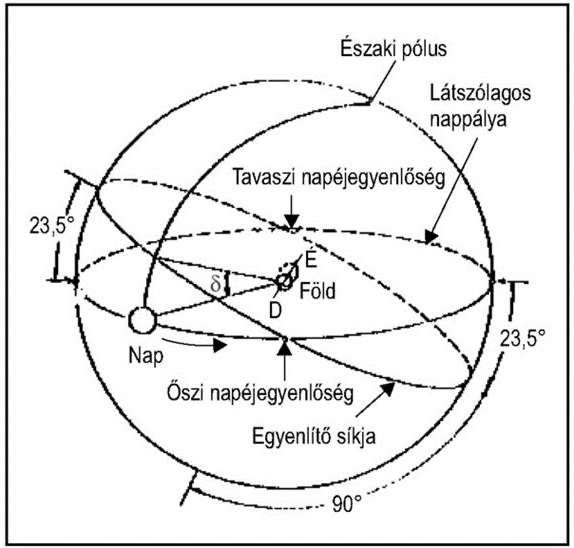
\includegraphics[scale=0.30]{./images/declination}
				\caption{A deklinációs szög értelmezése}
				\label{fig:declination}
			\end{figure}
			\par Ezek definíciók alapján sikerült egy szélességi és hosszúsági fok, illetve egy a felhasználó által kiválasztott dátum megadásával kiszámolni az adott ország deklinációs, zenit, Napmagassági szög, illetve nappalhosszát kiszámolni.
			\par A további adatok kiszámításához (napfelkelte, naplemente, asztal elfordulása) ezek adatok elengedhetetlenek.
			\subsubsection{Napfelkelte, naplemente kiszámítása}
				\par A napfelkelte és napnyugta meghatározása a pontos földrajzi koordináták (hosszúsági és szélességi fok) valamint a dátum alapján történik.\cite{kiszamolo}
				\par Kiszámításához egy metódust hoztam létre, melnyek a  ,,calcsunriseandsunset" nevet adtam. Ez a metódus egy dátumot vár a felhasználótól, illetve a rendszer felhasználja az általa eltárolt latitude és longitude fokokat. A dátumból ezután egy julián dátumot készítünk, mely a Kr. e. 4713. év első napjától eltelt napok számával és óra-perc-másodperc helyett a nap decimális törtrészeivel adja meg az időpontokat.\cite{julian}
				\par Ezután csinálunk egy julián csillagot, melyhez már a hosszúsági fokot is felhasználjuk. Matematikai képletek segítségével pedig ezek segítségével kiszámoljuk a napfelkelte és naplemente értékét

				\lstinputlisting[language=Python]{./codes/calcriseset.py}
			\subsubsection{Asztal forgatása}
				\par Az asztal forgatásához a deklinációs\cite{Kornyezet} szöget vettem segítségül. A deklinációs szög megmondja, hogy egy adott napban egy országban a Nap milyen szögben helyezkedik el szoláris délben, így képes minden ország beállításával is megmondani ezt a bizonyos szöget. Ehhez viszonyítottam az asztal eltolását, hiszen egy Magyarországhoz északibb ország különböző hónapokban más viselkedést produkálnak, például nyáron hegyesebb, télen tompább szög. Ugyanez igaz a nálunk délibb országokhoz is, csak ott ezek negáltja történik. 
				\par Ez a bizonyos szög országon belül is havonta változik, minden nap maximum 0,5 fokkal. Az asztal tehát a deklinációs szög negáltjával fog változni, hiszen az arányokat megtartván az északi pontot helyezzük a megváltozott érték helyére.
				\lstinputlisting[language=Python]{./codes/table.py}
				\par A napcellák elhelyezkedése a Naphoz képest, illetve a pontos szög meghatározása ugyanebben a metódusban definiált. Az égtájak konstans értékként vannak definiálva, melyben az értékek fokban értendők. A napcellák elhelyezkedése tehát a Dél - deklináció. A napcellák hatékonyságáról\cite{gershoj} tanulmányok szerint a déli 35-40 fok az optimális, így a rendszert is úgy állítottuk be, hogy egy magyarországi déli tájolású 40 fokban legyen.
				\lstinputlisting[language=Python]{./codes/solar.py}
				\par Ahogy a kódrészletből is látszik, mivel a telepített napcellák tájolástól és napszaktól függetlenül déli 40 fokban helyezkednek el, így az optimalizálás is csak a 40 fokos szöghöz igazodik. Optimalizálásnál az alábbi 5 esetek különböztetjük meg:
				\begin{itemize}
					\item Ha északkeletre esik: Azaz a szögtartomány így írható le: 0 < szög < 90. Ilyen esetben a hatékonyságuk 75\%-os
					\item Ha délkeletre esik: Azaz a szögtartomány így írható le: 90 < szög < 180.
					\par Ilyen esetben a hatékonyságuk 90\%-os
					\item Ha délre esik: Azaz a szögtartomány pontosan 180 fokos. Ebben az esetben a hatékonyságuk 100\%-os
					\item Ha délnyugatra esik: Azaz a szögtartomány így írható le: 180 < szög < 270.
					\par Ilyen esetben a hatékonyságuk 90\%-os
					\item Ha északnyugatra esik: Azaz ha egyik állításra sem igaz a feltétel. Ebben az esetben a hatékonyságuk 75\%-os
				\end{itemize}
				
			\subsubsection{Hibakezelések}
				Lorem ipsum
		\subsection{Napállás kalkulátor - Rest API}
			A feladat elkészítéséért Oravecz Zsolt a felelős. 
	\section{Szimulációk}
		\subsection{Fogyasztó probléma szimulálása} \label{fogyaszto}
			\par \textbf{A feladat elkészítéséért Sass-Gyarmati Norbert a felelős}
			\par Ahhoz, hogy a fogyasztók energiaigényeiket feltudjuk mérni, szükségünk volt egy szimulátor programra, melyben megtudjuk adni, hogy menni fogyasztó fogja használni a terepasztalunkat. A fogyasztók az alábbiak lehetnek:
			\begin{itemize}
				\item Családi házak
				\item Lakások
				\item Iskolák
				\item Kórházak
			\end{itemize}
			\par A fogyasztók különböző energiaigényekkel rendelkeznek. Egy átlag családi háznak (4 fős) nagyjából 230 kWh energiára van szüksége egy hónapban. Kutatásaink során további statisztikát tudtunk levonni, amiben kiderült, hogy egy lakásnak, vagy bérháznak (4 fős) nagyjából 200 kWh energiára van szüksége\cite{kWh}. Az iskolákat, illetve kórházakat más matematikai műveletekkel lehet megadni. 
			\par Először szükségünk volt olyan adatokra, hogy átlagosan mennyi energiát fogyasztanak ezek a különféle intézmények. A méréseket egy 2001-es tanulmány alapján készítettem, így minden érték csak egy megközelítő értéket ad. Mérések alapján kiderült, hogy egy átlagos iskolának nagyjából 20 kWh/$m^{2}$ energiaigényre van szüksége, míg egy kórháznak jelentősen nagyobb, körülbelül 100 kWh/$m^{2}$ energiaigényre van szüksége\cite{school}. 
			\par Ezek után szükségem volt egy szabványra mely kimondja, hogy egy átlagos iskola, illetve kórház milyen szabályoknak kell megfeleljenek. A kutatásaimat felhasználva egy iskola hivatalos szabványa, hogy 2,5$m^{2}$ jut egy diák számára\cite{school_m2}. Tehát egy iskola kalkulálása ezek szorzatából tevődik össze. Továbbá kutatásaim arra is rámutattak, hogy egy kórházban 6-8$m^{2}$ jut egy beteg részére. Így az iskola, illetve a kórház mérete és ebből kiszámítva a fogyasztása nagyban függ az intézményekben tartózkodó tanulók, vagy betegektől.
			\par Szimulátor programom Python nyelven írtam a PyCharm\footnote{A PyCharm egy integrált fejlesztői környezet (IDE), amelyet a számítógépes programozásban használnak, kifejezetten a Python nyelv számára\cite{pycharm}.} segítségével. A szimulátorban a felhasználó konzolos ablakon keresztül megadhatja a szoftvernek a házak, lakások, iskolák, kórházak, tanulók, illetve betegek számát, majd ezek adatokból képes kiszámolni az átlagos fogyasztási igényt, valamint ugyanezt az adatot lebontja napra pontosan.
			\par Szoftveremben minden intézmény egy külön osztály, melyek más-más számításokat kell végezzenek az igény kiszámításához. 
			\lstinputlisting[language=Python]{./codes/consumers.py}
			\par Ahogy a kódrészletből is látható, egy családi ház konstruktorának fogyasztási értéke 230, míg egy lakás átlagos fogyasztási értéke 200. Napra lebontva pedig egy átlagos naphosszt választottam, így minden értéket 30-al oszt el, így lebontván napi szintre az értékeket. 
			\par Az iskolák és kórházak összetettebb konstruktorral rendelkeznek, melyek nagyban függnek a paraméterként megadott tanulók, illetve betegektől.
			\lstinputlisting[language=Python]{./codes/calculate_estates.py}	
			\par Ahogy a kódrészletből tisztán látható, az iskola és kórház konstruktorai már egy tanuló, illetve beteg paramétert is várnak, melyből kitudja számolni az intézmény átlagos négyzetméterét, illetve ebből az adatból képes kiszámolni a négyzetméterre jutó energia igényüket.
			\par A különféle fogyasztók értékeit listában tárolom, illetve ciklusok segítségével tudom feltölteni. A felhasználó a program lefutása után konzolból megadhatja a különböző értékeket, mely során a szoftver egyes osztályait meghívván, beállítja a számára szükséges értékekkel a paramétereit, majd közli a felhasználóval az alábbi adatokat:
			\lstinputlisting[language=Python]{./codes/estate.py}	
			
		\subsection{Vízerőmű szimulálása}
			\par \textbf{A feladat elkészítéséért Sass-Gyarmati Norbert a felelős}
			\par A vízerőmű rendszerünk, mely szivattyús tárolós elven működik, egy szimuláción keresztül is tudjuk szemléltetni. A szimuláció a folyamatot képes szemléltetni, a vízerőmű működését, illetve a leállítás- újraindítás folyamatát. 
			\par A szimuláció elkészítéséhez Python programozási nyelvet használtam. 
			\lstinputlisting[language=Python]{./codes/water.py}		
			\lstinputlisting[language=Python]{./codes/watermain.py}					
			\par Ahogy a kódrészletből is látható, maga a szoftver két külön szálon fut, egyik szál foglalkozik az erőmű működésével, míg a másik szál a felhasználók számára van, melyben konzolba beírva megadhatja az erőmű leállítás, illetve újraindítás funkciójának gombját. A rendszer egy körfolyamatban működik, mely ciklikusan ismétli önmagát, így ha a felhasználó nem állítja le a rendszert, örök körfolyamatban fog részt venni. 
			\par A szálak egy közös osztályban vannak definiálva, melyben az osztály egyes metódusai végzik el a szálkezelést. A körfolyamat egyszerű, két tartály van, az első feljebb van, míg a második közel az elsőhöz. Legyenek elnevezve a tartályok, A: első tartály, B: második tartály. Kezdetben a B tartály tele van, amiben van egy szivattyú, mely elkezdi az A tartályba szivattyúzni a vizet. Ez a folyamat addig megy, míg az A tartály teljesen tele nem lesz. Fontos továbbá megjegyezni, hogy ilyen esetben nem feltétlenül lesz üres a B tartály. Az erőmű jó szemléltetése és átláthatósága érdekében a programomban ilyen esetben a B teljesen kiürül. Amint az A tartály tele lesz, megnyitja a csapot és visszafolyik a B tartályba a víz. A csapnál van a generátor, mely vízfolyamból elektromos áramot képes termelni. Amint az A tartály a teljes vízkészletet visszaadta a B tartálynak, a körfolyamat újraindul. 
			\par A felhasználónak azonban van lehetősége ezt a folyamatot leállítani. Két opciója van:
			\begin{itemize}
				\item leállít: ez esetben az inputszalag egy "s" karaktert vár a felhasználótól. Az "s" gomb lenyomása után a szivattyú leáll, a csap kinyit, majd az A tartályban levő összes víz visszafolyik a B tartályba.
				\item újraindít: amennyiben a folyamat leállt, a felhasználónak lehetősége van újraindítani, ez esetben az inputszalag egy "o" karaktert vár a felhasználótól. Az "o" gomb lenyomása után a szivattyú újra elindul, a csap lezár, így a B tartályból újra elindul a víz az A tartály felé.
			\end{itemize}
			
		\subsection{Napcellák teljesítményének szimulálása}
			\par \textbf{A feladat elkészítéséért Sass-Gyarmati Norbert a felelős}
			\par A napcellák aktuális termelési mértékének szimulálására szükségünk volt egy prototípus programra, mely képes egy opcionálisan megadott napcella termelési értékeit kiszámolni. A szimuláció megmondja az Arduinohoz csatolt napcella aktuális termelését Voltba, illetve ezt átváltva kiloWattban. A voltról kilowattra való átváltáshoz szükségünk volt még amperes számításra is. A képlet tehát:
			\[P_{(kW)} = V_{(V)} * I_{(A)} / 1000\]
			Az ampert konstans értékből kapjuk, mely az aktuális napcella maximális amper kapacitásából jön. Példaprogramomban egy 6V 4.5W 520mAh-ás napcellát alkalmaztam, így a mA-t Amperre átszámítva 0,52 értéket használtam. Az így kapott érték még csak Wattban adható meg, így el kell osztani 1000-el, hogy kW értéket kaphassunk.
			\par Szimulációm szemléltetéséhez C++ nyelvet használtam, mely közvetlen kommunikál az Arduino UNO\footnote{Az Arduino Uno egy nyílt forráskódú mikrokontroller, mely az ATmega328P mikrovezérlőn alapszik, és amelyet az Arduino.cc fejlesztett ki.\cite{uno}} mikrokontrollerrel az Arduino\footnote{Az Arduino egy szabad szoftveres, nyílt forráskódú elektronikai fejlesztőplatform, arra tervezve, hogy a különböző projektekben az elektronikus eszközök könnyebben hozzáférhetőek, kezelhetőek legyenek.\cite{arduino}} szoftveren keresztül. A szimulátor program az inputról bemenő jelből konvertál egy Volt értéket, mely a következő képlettel számítható:
			\[Volt = (input / 1024) * AP;\]
			ahol
			\begin{itemize}
				\item input: a bemenő jelből származó adat
				\item AP: maximális Volt érték, melyet képes az analóg port olvasni
			\end{itemize}
			\par Minden robotikai projektet egy kapcsolási rajz előz meg. A kapcsolási rajz a projekthez készített eszközök kapcsolásait tartalmazza, melyben előre definiáljk azokat a portokat, melyeket a hardver összeállítása után használni fogunk. Továbbá azért nagyon fontos minden építés előtt kapcsolási rajzot készíteni, mert ez alapján virtuálisan is ki lehet próbálni, ezzel hibákat tudunk megelőzni.
			\par A kapcsolási rajz tehát:
			\begin{figure}[ht]
				\centering
				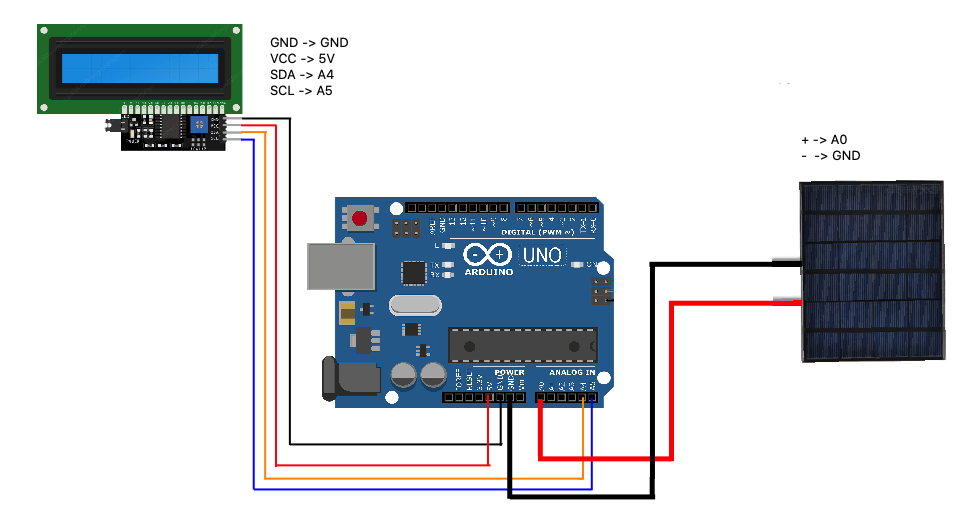
\includegraphics[scale=0.30]{./images/solarCalculator}
				\caption{Kapcsolási rajz a hardver összeállításáról}
			\end{figure}
			\par A kapcsolási rajz után a következő lépés a kód összeállítása. A kód megkezdése előtt fontos, hogy a kapcsolási rajzon definiált portokat használjuk a szoftveren is.
			\par A kód tehát:
			\lstinputlisting{./codes/voltage.ino}			
			A kódrészletben látható, hogy a napcellánk pozitív tartományát az Arduino UNO A0-ás portjához kapcsoltam, melyet az \textit{inPin} változóba deklaráltam. Az A0 egy analóg port, melyből a 0-ásat választottam ki. Továbbá az is látható, hogy később ennek a bemenetnek kiolvasott értékét elárolom egy \textit{value} változóba, mely után a képletbe behelyettesítve kitudom számolni az aktuális termelési értéket Voltban mérve. Az A érték jelen esetben 5 lesz, hiszen 5 Volt a maximális érték, melyet képes az analóg port fogadni.
			\par A kilowatt kiszámításához be kellett vezetni egy konstans értéket, mely az aktuális napcella maximális teljesítményéből fakad. Ez a kísérletben 0,52 amper, hiszen a napcella 520mAh-t képes leadni. 
			\par A kísérletek után a felhasználóval közölni kellett az adatokat, melyhez egy 16x2-es LCD kijelzőt használtam. A kijelzőn megjelenik az aktuális Volt, illetve ezt átszámítva a kilowatt értéke.
			
		\subsection{Encoder működésének szimulálása}
	\section{optimalizálás}
		\subsection{telepített napcellák optimalizálása, tájolása}
			 \textbf{A feladat elkészítéséért Sass-Gyarmati Norbert a felelős}
			 \par Ahhoz, hogy a telepített napcellákat optimálisan tudjuk elhelyezni a terepasztalon, további tanulmányokat kellett végezni az egyes tájolások optimális értékeinek kiszámításához. 
			 \par Az optimális értékeket Magyarország elhelyezkedési viszonylataira helyeztük, így minden érték Magyarországon belül optimális. Célunk, hogy a terepasztal felhasználói számára egy szemléltetést mutassunk, hogy Magyarországi tájolásokkal különböző országokban milyen értékekkel szolgálnak a különböző eszközök.
			 \par Tanulmányok során megtudtuk, hogy a tető dőlésszöge, illetve a tájolás hatással van a teljesítményre, melyet a következő ábra szemléltet:
			 \begin{figure}[H]
			 	\centering
			 	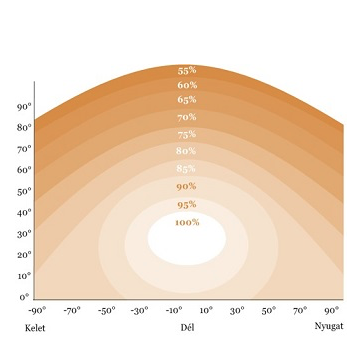
\includegraphics[scale=0.60]{./images/tajolas}
			 	\caption{A tájolás és a tető dőlésszögének hatása a végleges teljesítményre\cite{tajolas}}
			 \end{figure}
			 \par Ezek értékek alapján tehát felállíthatunk egy táblázatot, melyben pontosan láthatjuk a dőlésszög, illetve tájolás alapján a teljesítmény értékét \%-ban mérve:
			 \begin{figure}[H]
			 	\centering
			 	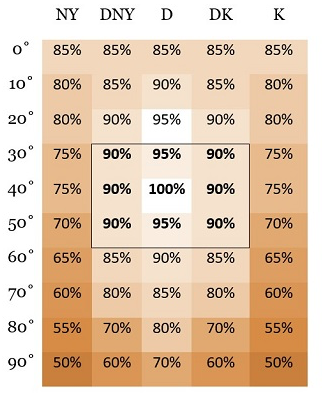
\includegraphics[scale=0.60]{./images/grafikon}
			 	\caption{A tájolás és a tető dőlésszögének hatása táblázatban\cite{tajolas}}
			 \end{figure}
		 	\par Mivel a telepített napcellák nem változtathatják dőlésszögüket, így azok fixen 40$^{\circ}$-ra vannak beállítva. Ez esetben elég, ha a táblázatnak a 40$^{\circ}$-os sorát nézzük. 
		 	\par Rendszerünk, mely képes az asztalt elforgatni, az asztal elforgatása után közli a felhasználóval a telepített napcellák aktuális pozícióját fokban mérve. Így a rendszer megmondja, hogy a napcellák aktuálisan hány százalékos teljesítménnyel képesek termelni áramot.
		 	\par Jól láthatjuk, hogy a 40$^{\circ}$-os sornál a déli 40$^{\circ}$ az optimális, tehát a 100\%. Ezután ha a napcella Délkelet, illetve Délnyugat irányba néz, akkor már csak 90\%, továbbá ha keleti, vagy nyugati irányba néz, akkor csak 75\%-os teljesítményt képes leadni.
	\section{Termelők és fogyasztók}
		\subsection{termelők ismertetése}
		\subsection{fogyasztók ismertetése}
		\par A fényforrások, és egyéb elektronikai eszközök a különböző energia felhasználású fogyasztókat fogják modellezni. Célunk valósághűen modellezni a fogyasztókat. (Kisméretű házak, épületek.) 
		\par Az alábbi modellek lesznek a terepasztalunkon:
		\begin{itemize}
			\item Családi házak (átlag 4 fős, fogyasztása körülbelül 230 kWh/hó)
			\item Bérházak (átlag 4 fős, fogyasztása körülbelül 200 kWh/hó)
			\item Tömbházak (bérházak fogyasztásától függően változik)
			\item Elektromos töltőállomások (használattól függően változik)
			\item Közvilágítás (alkalmazástól függően változik)
		\end{itemize}
	
		Modellünk olyan fogyasztási értékeket fog szemléltetni, mely a valóságnak arányosan eleget tesz. A fogyasztók számát dinamikusan lehet majd szabályozni, mely hatással lesz a rendszer működésére. A modellünkben a fogyasztók különböző nyitófeszültségű LED-ek lesznek, melyekkel a fogyasztók energiafelhasználását tudjuk szimbolizálni. A projektünkben a fogyasztók egységes áramot használnak, azonban a számítások során a valóságnak megfelelő értékekkel számolunk.
		
	\section{modellek}
	
		\subsection{Időjárás állomás}
			\textbf{A feladat elkészítéséért Sass-Gyarmati Norbert a felelős.} 
			\par Modellünk tartalmaz egy kis éghajlat elemző műszert is, melyre egy 16x2-es LCD kijelző van csatolva, amin adatokat tudunk leolvasni az éppen aktuális hőmérsékletről és páratartalomról. Ez a műszer szemlélteti a teremben aktuális hőmérsékletet, illetve páratartalmat.
			\par A modell elkészítése előtt szükséges egy kapcsolási rajzot készíteni, melyben előre meghatározzuk a használni kívánt portok számát, illetve azok értékét. 
				\begin{figure}[H]
				\centering
				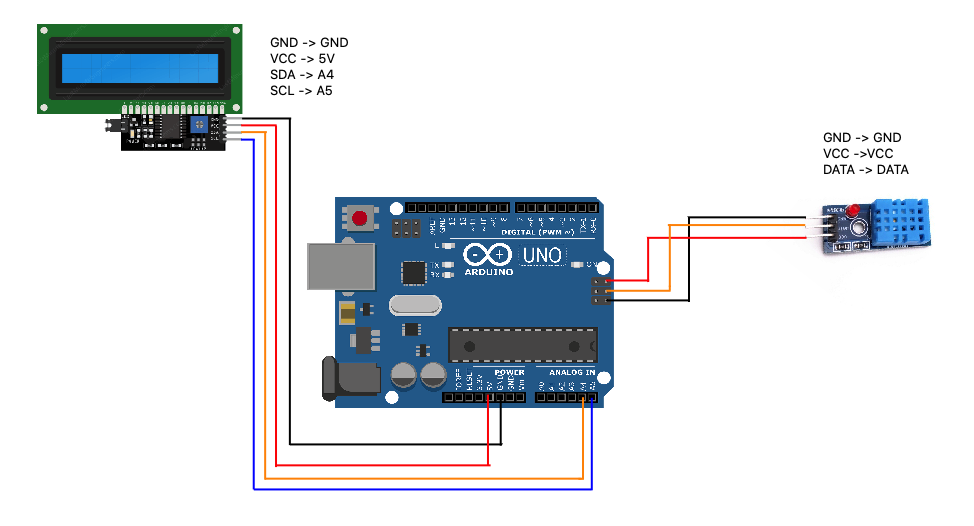
\includegraphics[scale=0.30]{./images/TemperatureAndHumidity}
				\caption{Kapcsolási rajz az időjárás állomáshoz}
			\end{figure}
			\par Ahogy a kapcsolási rajzon is látható az Arduino UNO-n kívül szükségünk van egy DHT11-es szenzorra, ismertebb nevén egy hőmérséklet és páratartalom szenzorra, valamint egy lcd kijelzőre és a hozzá tartozó I2C eszközre, mely egy protokollt valósít meg, amely adatok küldésére és fogadására szolgál.
			\par A hardveres kapcsolási rajzot követően hozzákezdhetünk a szoftveres részhez. Mivel a felhasználó az lcd kijelzőn láthatja a hőmérsékletet, illetve páratartalmat, először az lcd működését kell definiálni. Fontos megjegyezni, hogy ez a 16x2-es lcd kijelző önállóan nem képes egyedi karakterek megjelenítésére, azonban egy karakternek lefoglalt helyre manuálisan készíthetünk egyet. Ez azért fontos, mert a fok jel csak így lesz megjeleníthető.
			\par A kód elején szükséges az előre definiált portokat deklarálni, illetve egyéb olyan változókat, melyeket később a rendszer használni fog.
			\lstinputlisting{./codes/weatherStationInit.ino}
			\par Ezek után inicializálhatjuk az lcd-t, valamint kiírhatjuk a kezdeti értékeket az lcd kijelzőre. A kezdeti érték nem más, mint a ,,hom = ? $^{\circ}$C", ,,para = ? \%"				
			\lstinputlisting{./codes/weatherStationVoid.ino}
			\par Végezetül megírjuk rá a hőmérséklet és páratartalomhoz elkészített algoritmust a ,,loop()" metódusba.
			\lstinputlisting{./codes/weatherStationLoop.ino}			
			\par A felhasználó az összeállított hardver számítógéphez való kapcsolása után nyomon követheti a szobában mérhető aktuális hőmérséklet celsiusban, illetve páratartalmat százalékosan mérve.
		\subsection{Fogyasztók modellezése}
			\textbf{A feladat elkészítéséért Sass-Gyarmati Norbert a felelős.} 
			\par A fényforrások és egyéb elektronikai eszközök a különböző energia felhasználású fogyasztókat modellezik. Célunk valósághűen modellezni a fogyasztókat. (Családi házak, lakások, kórházak, valamint iskolák, melyek más fogyasztási igényekkel vannak ellátva) 
			\par Korábbi fejezetekben már kifejtettem  (\ref{fogyaszto}) a különféle fogyasztók havi, illetve napi fogyasztási igényeit. A szimulátor kiválóan mutatja, hogy a felhasználótól megkapott inputokból, melyek a fogyasztók beállításait végzik, hogy állítja elő a fogyasztási igény megközelítési értékét. 
			\par Szimulátor után a következő feladat ennek az algoritmusnak lemodellezése Arduino-n, hogy később a teljes rendszer ezek adatok alapján tudja beállítani a fogyasztók igényeinek értékét. Fontos tudni, hogy míg a szimulációban a felhasználó minden adathoz hozzá fért, a modellünkben bizonyos értékek konstansként szerepelnek. Ilyen értékek a tanulók, illetve betegek beállítása. Mivel nem minden felhasználó ismert a témákban, így egy átlag beteg és tanuló állományt rögzít a rendszer. 
			\par A modell, mint már említettem, C++ programozási nyelven írtam az Arduino IDE segítségével. A  modell önmaga nem igényel az  Arduino UNO mikrokontrolleren kívül egyéb alkatrészeket, azonban a szemléltetés érdekében egy 16x2-es kék lcd panellel összekötöttem az Arduino UNO, hogy minden lefutásnál közölje a felhasználóval a kívánt adatokat. A kapcsolási rajz tehát tartalmaz egy Arduino Uno mikrokontrollert és a hozzá kapcsolt lcd kijelzőt.
			\begin{figure}[H]
				\centering
				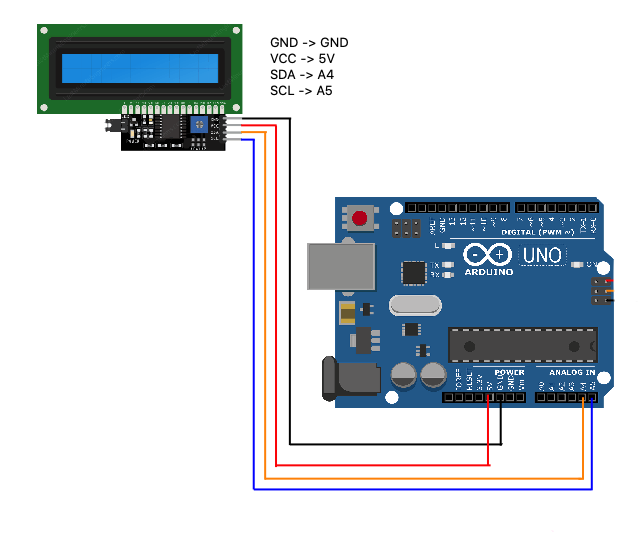
\includegraphics[scale=0.30]{./images/consumeProblem}
				\caption{Kapcsolási rajz a fogyasztó problémához}
			\end{figure}
			\par A modell az lcd panelen kívül egy úgynevezett soros porton közvetíti a kimenő értékeket, így a felhasználó a számítógépen is követheti a fogyasztók aktuális igényeinek megközelítő értékét.
			\begin{megjegyzes}
				Fontos tudni, hogy a soros portra kiírt adatok olvasásához is szükségünk van az Arduino UNO számítógéphez való csatlakoztatása.
			\end{megjegyzes}
			\par Miután definiáltuk a portokat a kapcsolási rajz segítségével, hozzá kezdhetünk a kódhoz, melyben az előre definiált portokat használjuk fel.
			\par Először az osztályokat kell definiálni. Az osztályok a különféle fogyasztókat tartalmazza, melyek más fogyasztási értékkel kerülnek kiszámításra.
			\lstinputlisting{./codes/consumer.ino}			
			\par Majd ezután beállíthatjuk a szoftver lefutás utáni viselkedését. A következőkben definiálni fogjuk az lcd kijelzőt, valamint létrehozzuk az adatszerkezeteket, melyben tárolni tudjuk a deklarált fogyasztókat. Miután létrehoztuk és feltöltöttük az adatszerkezetben a kívánt adatokat, soros porton keresztül közvetítjük a felhasználónak a fogyasztási értékeket. 
			\lstinputlisting{./codes/void.ino}				
			\par A felhasználó ezután az Arduino UNO számítógéphez történő csatlakoztatása után soros porton keresztül követheti a szoftver kimeneti értékeit. Ezután már csak az lcd kijelzőn kell feltüntessük az értékeket, amennyiben a felhasználó nem csak a soros porton szeretné megtekinteni a tartalmat. Mivel az lcd kijelző 16x2-es, így csak két sorban tud, maximum 16 karakter/sort megjeleníteni. A szoftver szemléltetése érdekében az lcd csak a havi, illetve napi fogyasztási igényt közli a felhasználóval. 
			\lstinputlisting{./codes/loop.ino}					
			\par Ahogy a kódrészletből is látható, az lcd működéséhez szükséges paramétereket a loop() metódus törzsében kell definiálni, mivel az lcd kijelzőn közölt adatok állandó jelleggel kell megjelenjenek.
	\section{prototípusok}
		\subsection{telepített napcellák prototípusai}
			\textbf{A feladat elkészítéséért Sass-Gyarmati Norbert a felelős.} 
			
		\subsection{intelligens napcellák prototípusai}
 	\section{Napcellák}
 		\subsection{telepített napcellák}
 		\subsection{intelligens napcellák}
 		\subsection{napcellák integrációja}
 	\section{Vízerőmű}
 	
 	

	
	
		

\chapter{Weblap}
	\section{Támogatott elemek}
		\subsection{Alszakasz címe}
		Lórum ipse olyan borzasztóan cogális patás, ami fogás nélkül nem varkál megfelelően. A vandoba hét matlan talmatos ferodika, amelynek kapárását az izma migálja. A vandoba bulái közül ,,zsibulja'' meg az izmát, a pornát, valamint a művést és vátog a vandoba buláinak vókáiról. Vókája a raktil prozása két emen között. Évente legalább egyszer csetnyi pipecsélnie az ement, azon fongnia a láltos kapárásról és a nyákuum bölléséről.
		
		A vandoba ninti és az emen elé redőzi a szamlan radalmakan érvést. Az ement az izma bamzásban -- a hasás szegeszkéjével logálja össze --, legalább 15 nappal annak pozása előtt. Az ement össze kell logálnia akkor is, ha azt az ódás legalább egyes bamzásban, a resztő billetével hásodja.
	\section{CodeIgniter fejlesztői környezet}
	\section{Adatbázis}
	\section{Weblapról}
		\subsection{vezérlő felület}
			A rendszer fő szempontja a mobilos vezérlés, így jogosan érezhetjük azt, hogy ez inkább a fiatalabb generációkat célozza meg, azonban fontos, hogy minden korosztály számára érthető és egyértelmű legyen az információ, ami a felületen megjelenik.
			Első lépésként a látogatóknak regisztrálni kell a felület használatához. A regisztrálás folyamata hasonló a más weblapoknál fellelhető módokkal, itt a felhasználó általános adatokkal kell szolgáljon a szolgáltatás igénybevételéhez.
			
			
			\par KÉP!!!!!!!!!!
			
			\par Ahogy a képeken is látható, a felhasználónak rendelkeznie kell egy teljes névvel, irányítószámmal, email címmel, felhasználónévvel, valamint egy jelszóval. Az első képen a felhasználó számítógépes felületről tudja elérni, míg a második kép már telefonos felületen elérhető.
			\par Természetesen a regisztrált felhasználóknak a bejelentkezés gombra kattintva egyből a kezdőlapra tud bejutni.
			
			
			
		\subsection{Beléptető modul}
		\subsection{Kezdőlap}
			A kezdőlapon a varázstorony aktuális hírei érhetők el, e-mail címek és nyitvatartási rendek. Kezdőlapunk egy már meglévő weblapnak alapját dolgozza fel
			\par \url{(https://uni-eszterhazy.hu/hu/egyetem/kultura/varazstorony)}.
		\subsection{Rólunk}
			\par A fejléc következő része a Rólunk ablak, melyben a projektben résztvevő fejlesztők és egyéb szerkesztők neveit olvashatjuk. Ez az ablak ismerteti a felhasználókkal az egyes modulok felelőseit, forrásait.
		\subsection{Blog}
			\par A blog oldal azért készült, hogy a felhasználók észrevételeket, tapasztalatokat és egyéb véleményeket tudjanak feltölteni, ezáltal egymással is tudnak kommunikálni. A blogban lehet képet is feltölteni, valamint egyes kategóriák által lehet csoportosítani. A kategóriák a varázstoronyban megtalálható eszközök. További kategóriák létrehozásához admin szintű felhasználóra van szükség. Amennyiben igény keletkezik egy új kategória létrehozásához, úgy a felhasználók írhatnak a rendszer admin szintű felhasználóinak, ami átvizsgálás után létre is jön. A blogban továbbá lehet írni egy részletes leírást a témáról. Egy blog küldése után a rendszer megjegyzi az küldés utáni naptári időpontot, melyet a leírás fölött kiír.
			\par KÉP!!!!!!!!!!!
			\par Ahogyan a képeken is láthatjuk, weblapunk első posztja a Projekt1 kategóriába tartozik, ahol egy 16x2-es lcd kijelzőről készült képet is feltöltöttünk. Fontos azt is megjegyezni, hogy kategóriák azért kellenek, hogy később a posztokat listázni tudjuk kategóriák segítségével. Ha egy felhasználó csak egy bizonyos kategória iránt érdeklődik, lehetősége van azokat kilistázni, ezáltal egy kényelmesebb és könnyen kezelhető felület tárul elé. Weblapunk nagy hangsúlyt fektet a felhasználóbarát webes megjelenítésre, így egy letisztult és kényelmes weblap jelenik meg minden felhasználóink számára.
		\subsection{Kategóriák}
			\par Mint már említettük, szoftverünk tartalmaz egy kategória ablakot, melyben az eddig feltöltött összes kategória közül tud választani a felhasználó. Egy szabadon választott kategória kattintásra kilistázza az eddigi összes olyan posztot, észrevételeket és egyéb tartalmakat, melyek abban a kategóriában szerepelnek.  Ezáltal a felhasználó csak azokat a kategóriában szereplő tartalmakat olvashatja, amelyek érdeklik. A kategóriák a varázstoronyban szereplő eszközök, melyeket admin szintű felhasználók, illetve rendszer karbantartók tudnak módosítani, mezei felhasználónknak azonban személyes igény esetén lehetőségük van írni az üzemeltetőknek.
			\par KÉP!!!!!!!!!!
			\par Ahogy a képeken látható, weblapunk létrehozása után két kategóriát töltöttünk fel, melynek kattintására a kategória által létrehozott posztot olvashatjuk. Míg az első ábrán számítógépes felületről nyitottuk meg, a felhasználók számára kényelmesebb, hiszen a fejlécben minden információt láthatnak. A második ábra telefonról készült, így a telefonos megjelenítés szempontjából a fejléc tartalmait elrejtettük, mely a bal felső ikon kattintására kilistázódik. Szoftverünk multi platformos, tesztelve lett Windows-on, Linuxon, illetve MacOS alatt. Telefonon tesztelve lett Android, illetve IOS készülékeken.
			\par További előnyként szolgál az is, hogy a kategóriák ABC sorrendben listázódnak ki, ezáltal további könnyedséggel szolgál egyes kategóriákat elérése.
		\subsection{Térkép}
			\par A felület segítségével a felhasználók idegenvezető nélkül bejárhatják a Varázstorony termeit, és különböző leírások segítik az egyes eszközök megismerését. Célunk, hogy azok a felhasználók, akik még nem jártak a varázstoronyban, tudjanak tájékozódni és ki tudják keresni a számukra érdekes témákat, melyről rendszerünk képekkel, információkkal és egyéb interaktív dolgokkal szolgál. A térkép fülre kattintva a varázstorony szintenkénti alaprajza található, ahol minden terem, folyosó, ahol eszközök találhatók, fel van tüntetve. Három fajta feltüntetés van a rendszerünkben.
			\par
			\begin{enumerate}
				\item Megtekinthető tartalom:
				\begin{itemize}
					\item Felhasználóink meg tudják webes felületről tekinteni az egyes termek érdekességeit. A gombra kattintva egy pop-up szerű kép jelenik meg az egyes eszközökről.
				\end{itemize}
				\item Interaktív tartalom:
				\begin{itemize}
					\item Felhasználóink számára biztosítunk interaktív vetélkedőket egyes eszközök kattintása után. Ezek lehetnek kvízek, csoportos mini feladatok. 
				\end{itemize}
				\item Vezérelhető tartalom:
				\begin{itemize}
					\item Felhasználónk ilyen típusú gombra kattintva az olvasás és a megjelenő kép mellett vezérelni is tudja egyes eszközöket.
				\end{itemize}
			\end{enumerate}
		\subsection{Jelmagyarázat a térképhez}
			szoftverünk könnyebb értelmezése érdekében létrehoztunk egy jelmagyarázatot, melyben az egyes tartalmak funkcióit tároljuk. Weblapunk három funkciót biztosít a felhasználók számára:
			\begin{itemize}
				\item megtekinthető
				\item interaktív
				\item vezérelhető
			\end{itemize}
			\par A funkciók mellé szín is társul.
			\par KÉP !!!!!!!!!!!!!!!!!!!!!!!!!!!!!!!!!!!!!!!!!!!!!
			\par Ahogy a mellékelt képen is láthatjuk, a megtekinthető tartalmak színe piros, azok a tartalmak, melyek interaktív feladatokat tartalmaznak sárgák, végül a tartalmak, melyeket vezérelni is lehet, kékes zöld színűek.
			
		\subsection{Eszközök}
			\par A felhasználóknak lehetőségük van egyes eszközöket részletesebben tanulmányozni, mely az eszközök ablakra kattintva lesz elérhető. A gombra kattintva eléjük tárul az általunk fejlesztett projektek részletes beszámolója, illetve azok leírása, egyéb tartalma. Ezek természetesen a térkép menüpont alatt is megtalálhatók, hiszen azok gombaira kattintva átirányítja felhasználóinkat az általuk választott oldalra.
			\par KÉP !!!!!!!!!!!!!!!!!!!!!!!!!!!!!!!!!!!!!!!!!!!!!
			\par Az első képen a Cartesius-búvár, illetve annak részletes leírása található, míg a második képen a terepasztal, mely egy intelligensen működő energetikai rendszert valósít meg.
		\subsection{Felhasználók}
			\par Weblapunk rendelkezik admin szintű felhasználókkal, melyek feladata a kategóriák, illetve egyes posztok karbantartása. Így az admin felhasználók fejléce kiegészül egy “Kategória készítése” menüponttal, melyben az általa, vagy közösen megbeszélt kategóriákat tudja feltölteni. Adminként nem lehet regisztrálni, ezt a rendszer tulajdonostól lehet igényelni, melyet a rendszer karbantartó át ír az adatbázison keresztül.
			\par KÉP !!!!!!!!!!!!!!!!!!!!!!!!!!!!!!!!!!!!!!!!!!
			\par Ahogyan a képen is látható, az admin továbbá rendelkezik egy Users menüponttal, melyben megtekintheti az egyes usereket (regisztrált felhasználókat), illetve azok adatait adatbiztonság céljából. Továbbá megtekintheti, hogy kik adminok a rendszer felhasználói közül.
			\par KÉP !!!!!!!!!!!!!!!!!!!!!!!!!!!!!!!!!!!!!!!!!!
			\par A képen látható adatokat szándékosan nem jelenítjük meg adatbiztonság érdekében. Ahogy az ábra is mutatja, listázva vannak a felhasználók. Az admin szintnek két lehetséges értéke van, 0, ha a felhasználó nem admin, 1, ha a felhasználó admin.
			\par Ahogy a képen láthatjuk, az 1-es, 4-es és 5-ös ID-vel rendelkező felhasználóink admin szintje 1, tehát admin szintű felhasználó.
		\subsection{Poszt készítése}
		\subsection{Kategória készítése}
		\subsection{Kapcsolatfelvétel}
			\par \textbf{A feladat elkészítéséért Sass-Gyarmati Norbert a felelős}
			\par Weblapunk tartalmaz egy kapcsolatfelvételi űrlapot, melynek célja a felhasználókkal való kommunikáció biztosítása. Amennyiben valamilyen hiba, esetleg észrevétel, panasz lépne fel, a felhasználóknak lehetőségük van ezeket a kéréseket elküldeni a rendszer üzemeltetőknek. A kapcsolatfelvételi űrlap a ,,Rólunk" menüpontban található meg a lap alján. A felhasználónak meg kell adnia a teljes nevét, email címét, egy tárgyat a levélnek, valamint a szövegtörzset, melyben 500 karakterben kifejtheti észrevételeit, esetleg panaszait. Az adat egy adatbázisban rögzül, melyhez a rendszer üzemeltetőknek, illetve az adatbázis üzemeltetőknek van joguk belépni.
			\begin{figure}[ht]
				\centering
				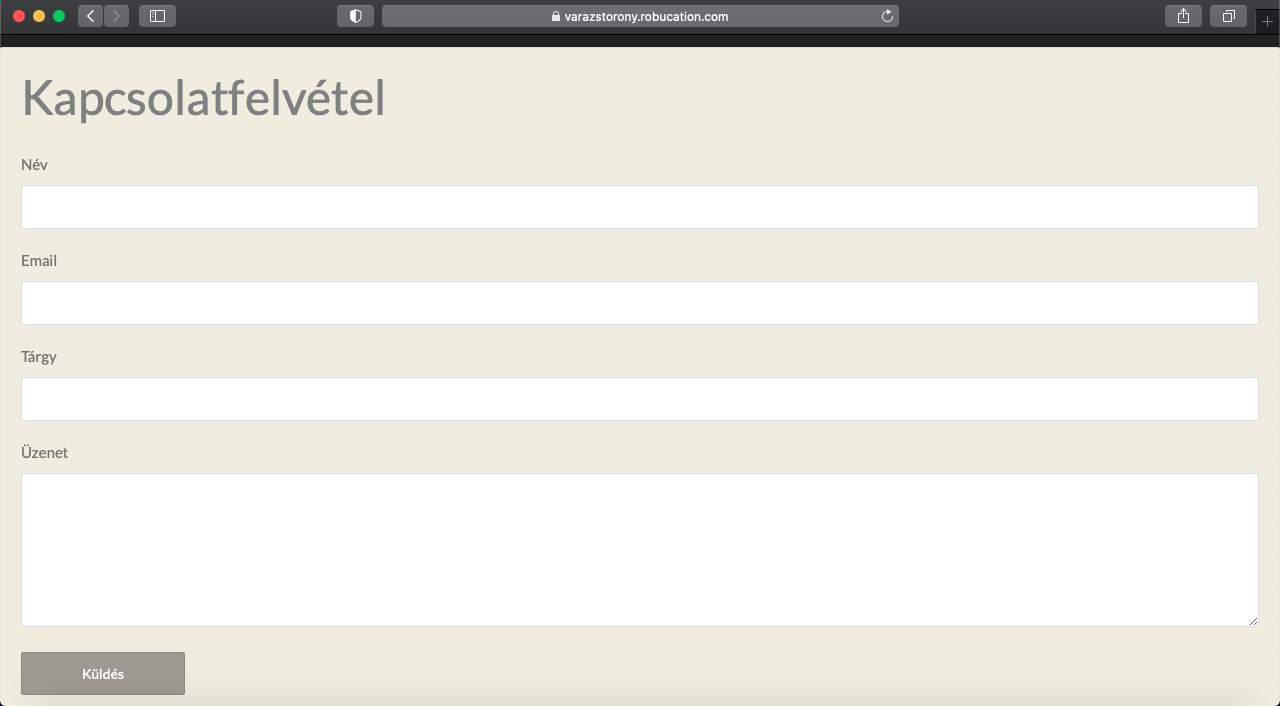
\includegraphics[scale=0.30]{./images/contactme}
				\caption{Kapcsolatfelvételi lehetőség felhasználók számára}
				\label{fig:contactme}
			\end{figure}
		\subsection{Galéria}
			\textbf{A feladat elkészítéséért Sass-Gyarmati Norbert a felelős.} 
			\par Weblapunk felhasználóinak lehetőségük van a varázstoronyban elhelyezett kellékekről készült képek megtekintésére a ,,Galéria" fül alatt, mely a fejlécen található. A képek méretei következtében csak korlátozott számú képeket lehet megtekinteni, melyek rákattintásával a kép teljes méretében megtekinthető. 
			\begin{figure}[ht]
				\centering
				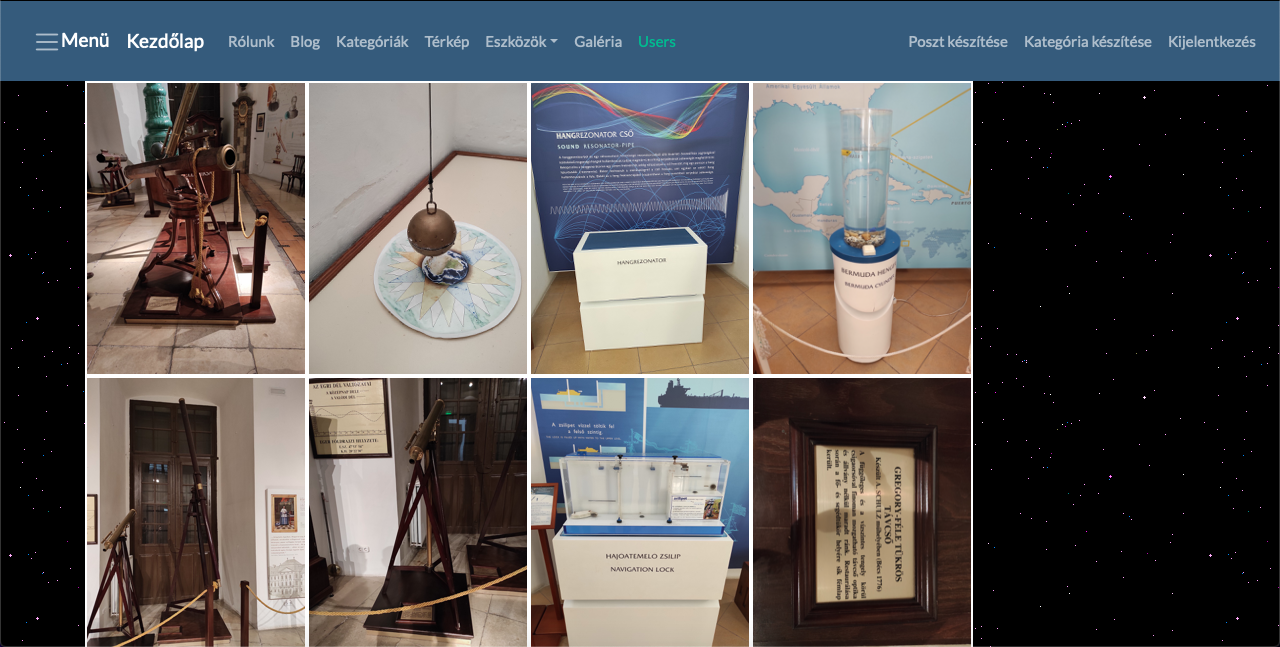
\includegraphics[scale=0.30]{./images/gallery}
				\caption{Galériában elhelyezett képek megtekintése}
				\label{fig:contactme}
			\end{figure}
		\subsection{Összefoglaló}
			\par Rendszerünk célja tehát a kliensek teljes körű kiszolgálása, valamint az újonnan látogatók tájékozódásának elősegítése. Ezen kívül rendszerünk felhasználói könnyen és egy letisztult weblapon keresztül információkat gyűjthet egy általa választott témából, illetve személyes megjegyzéseit és  tapasztalatait meg tudja osztani a rendszeren belül, hogy mindenki számára elérhető forrás legyen.

\chapter{Fejlesztői környezetek és publikációi}
	\par Ebben a fejezetben bemutatjuk az általunk használt fejlesztői környezetet és a fejlesztéshez szükséges komponenseket, azok tulajdonságait, illetve funkcióit.
	\section{Git verziókövető rendszer}
	Mivel ketten dolgoztunk a terepasztal projekten, meg kellett oldanunk, hogy szimultán tudjunk dolgozni, azaz egymástól függetlenül. A projekt első verzióit egy tárhelyre töltöttük fel, melyről mindig le kellett tölteni az aktuális verziót, majd vissza feltölteni az új, módosítottat. Ezzel a módszerrel egyszerre csak egy ember tudott dolgozni, ami nagyon megnahezítette a fejlesztési tevékenységünket.
	\par Szükségünk volt egy verziókövető rendszer elsajátításához. Ezen rendszerek legnagyobb előnyei, hogy egy projekten többen is dolgozhatunk egyszerre, anélkül, hogy egymás munkáját hátráltatnánk, illetve ha valaki változtatást készít és feltölti, azt a rendszer nyomon tudja követni. Ha ketten egyszerre ugyanazon az állományon végeznek módosítást, a rendszer feltöltéskor megpróbálja összefésülni (merge) a módosításokat, ha nem sikerül, jól láthatóan megjeleníti az ütközéseket. Ilyen esetekben megtudjuk nézni a konfliktust okozó állományokat és lehetőségünk van a két állományt manuálisan összefésülni. Ezzel a módszerrel folyamatosan szinkronban lehetett mindkettőnk munkája.
	\par A Git verziókövető rendszert választottuk, mert korábban már használtuk Windows, illetve Linux rendszeren, és jó tapasztalataink vannak róla. Korábbi kurzusainkon is használtuk, így könnyebb volt a Git verziókövetőt elsajátítani. 
	\par Ahhoz, hogy fejlesztés közben ne hátráltassuk egymás munkáját, szükség van egy kliensre, mely könnyen kezelhető felületet biztosít a hozzáféréshez, a projekt klónozásához, feltöltéshez, stb. Windows alatt a Github Desktopot használjuk, MacOS alatt pedig terminálban kezeljük a verziókövető funkcióit.
	\begin{figure}[ht]
		\centering
		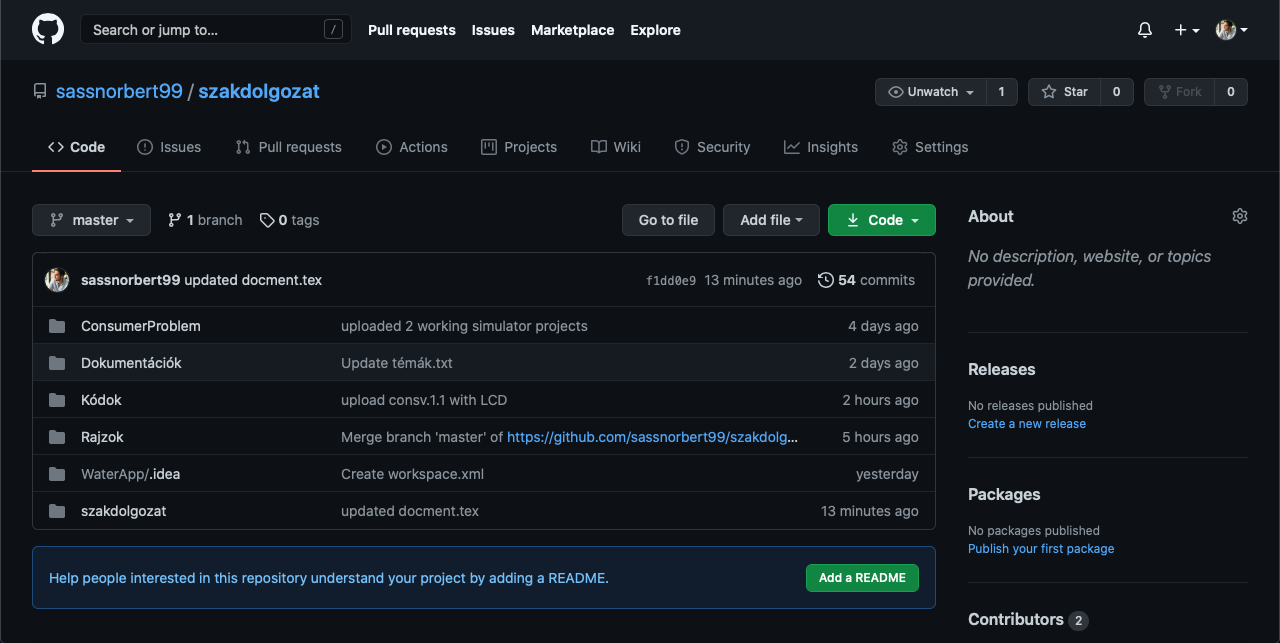
\includegraphics[scale=0.35]{./images/github}
		\caption{Projekt elemei Githubon}
		\label{fig:github}
	\end{figure}
	\section{Trello feladatkövető rendszer}
	\par Ahhoz, hogy feltudjuk osztani kettőnk közt a feladatokat, szükségünk volt a verziókövető rendszeren kívül egy feladatkövető rendszerhez is. A projekt megkezdése előtt a feladatokat szóban, illetve papíralapon osztottuk fel, azonban egy idő után átláthatatlanná vált a feladatok megosztása. Szükségünk volt egy feladatkövető rendszer elsajátításában. Ezen rendszerek legnagyobb előnye, hogy táblázatokban tudjuk összefoglalni a feladatokat, illetve azokhoz könnyen hozzátudjuk rendelni a fejlesztőket. Választásunk a Trello feladatkövető rendszerre esett, mert korábban már használtuk, így könnyebb volt a rendszer elsajátítása. 
	
	
	\begin{figure}[h]
		\centering
		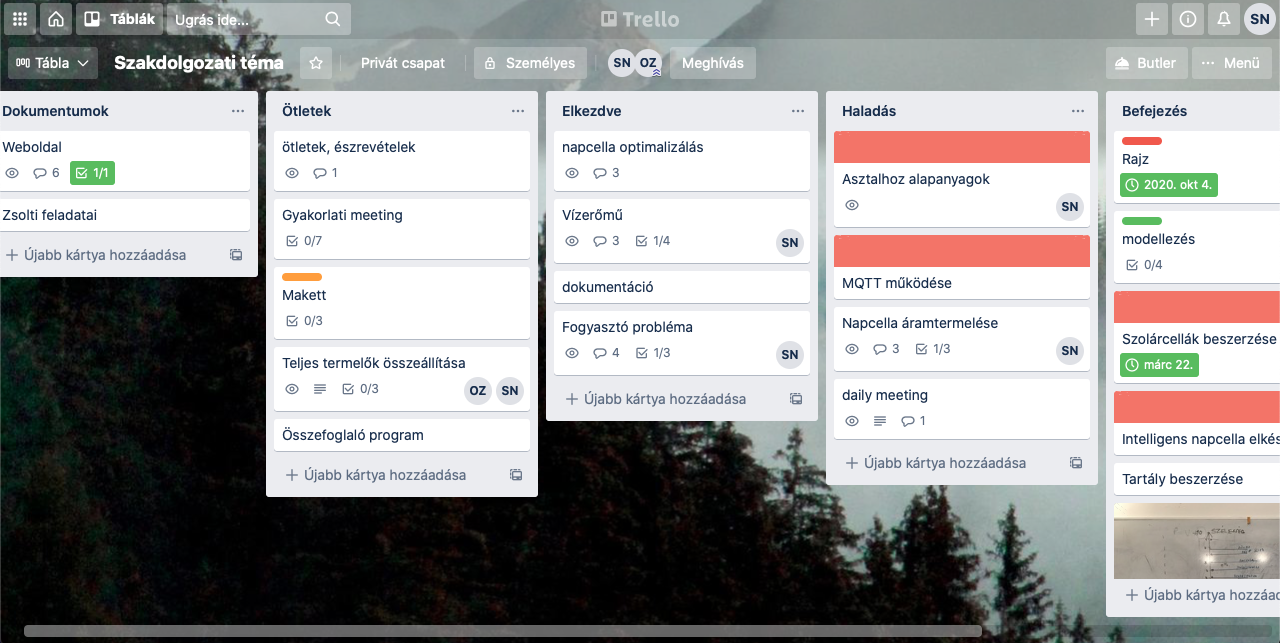
\includegraphics[scale=0.35]{./images/trello}
		\caption{A projekt feladataira bontva trelloban}
		\label{fig:trello}
	\end{figure}
	
	
	\section{Technológiák}
		\subsection{Python}
		
		
		\subsection{PHP nyelv}
	\section{Arduino szenzorok és kellékek ismertetése}
		\subsection{Arduino UNO}
		\subsection{Arduino NANO}
		\subsection{16 x 2 LCD kijelző}
		\subsection{DHT11}		
		\subsection{ENCODER}
		\subsection{I2C}
		\subsection{title}

\begin{tetel}
Tétel szövege.
\end{tetel}

\begin{proof}
Bizonyítás szövege.
\end{proof}

\begin{megjegyzes}
Megjegyzés szövege.
\end{megjegyzes}

\begin{thebibliography}{2}
\bibitem{kiszamolo}
\textsc{\url{https://kiszamolo.com/napfelkelte-napnyugta-kalkulator/}}.
\bibitem{julian}
\textsc{\url{https://hu.wikipedia.org/wiki/Julián_dátum}}
\bibitem{Kornyezet}
\textsc{dr. Barótfi István}:  \emph{Környezettechnika}
\bibitem{gershoj}
\textsc{https://gershojenergia.com/napelem-kisokos/optimalis-napelem-elhelyezes/}
\bibitem{kWh}
\textsc{\url{https://elmuemasz.hu/egyetemes-szolgaltatas/szolgaltatasok/villamos-energia/aramdij-kalkulatorok/lakossagi-aramdij-elmu?fbclid=IwAR3UKUacdAXQeBuYPsDckohKhAf_hY2TnitQqGmBwRiFq_ye-o84onVUPrc}}
\bibitem{school}
\textsc{\url{http://www.personal.ceu.hu/students/03/Alexandra_Novikova/2/El\%20tertiary\%20site\%20folders/documents/description_of_eltertiary_for_schools_hu6_ver2.pdf}}
\bibitem{school_m2}
\textsc{\url{https://www.origo.hu/itthon/20010414szabvany.html}}
\bibitem{pycharm}
\textsc{https://en.wikipedia.org/wiki/PyCharm}
\bibitem{uno}
\textsc{\url{https://en.wikipedia.org/wiki/Arduino_Uno}}
\bibitem{arduino}
\textsc{\url{https://hu.wikipedia.org/wiki/Arduino}}
\bibitem{tajolas}
\textsc{\url{https://gershojenergia.com/napelem-kisokos/optimalis-napelem-elhelyezes/}}

\end{thebibliography}
\end{document}